\documentclass{beamer}
\usetheme{Warsaw}
\usepackage{ragged2e}
\usepackage{multimedia}
% \usepackage{english}
\usepackage[utf8]{inputenc}
\usecolortheme{beaver}
\title[]
{Documents classifier}
\author[] {Tomasz Kulik}
\date[2019]
{2019}
\subject{Machine Learning}


\begin{document}
    \begin{frame}
        \titlepage
    \end{frame}


    \section{Introduction}
    \begin{frame}
    	\frametitle{Next chapter}
        \tableofcontents[currentsection]
    \end{frame}
    \begin{frame}
        \frametitle{Who am I}
        \begin{center}
            Tomasz Kulik
        \end{center}
        \begin{itemize}
            \item Software Developer in Nokia
            \item MSc in Computer Science, graduated from University of Science and Technology in Wrocław
            \item Interested in programming, algorithms, machine learning
        \end{itemize}
    \end{frame}
    \begin{frame}
        \frametitle{Scope of the presentation}
        Documents classifier
        \begin{itemize}
            \item Information about the dataset
            \item Text preparation
            \item TF-IDF method desciption
            \item Reccurent Neural Network method desciption
            \item Application
        \end{itemize}
    \end{frame}

    \section{Description of tools / dataset}
    \begin{frame}
    	\frametitle{Next chapter}
        \tableofcontents[currentsection]
    \end{frame}
    \begin{frame}
        \frametitle{Dataset}
        \begin{itemize}
            \item 18846 documents
            \item 20 subjects
            \item 83\% of data used as training set
        \end{itemize}
    \end{frame}
    \begin{frame}
        \frametitle{Dataset}
        \centering
        Distribution of the dataset:
        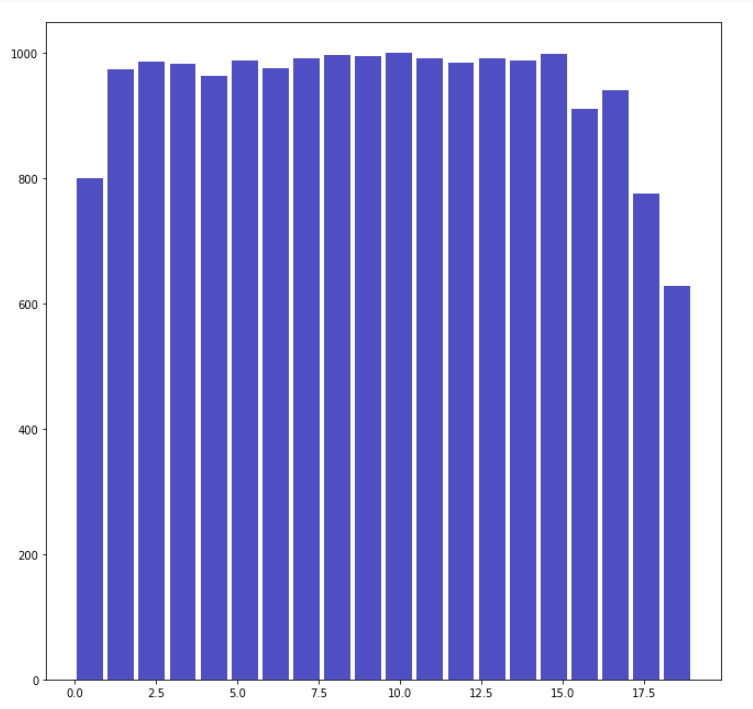
\includegraphics[width=0.6\textwidth]{data_distribution.png}
    \end{frame}
    \begin{frame}
    	\frametitle{Tools}
        \begin{itemize}
            \item Python 3 - Keras, SciKit learn, NLTK, (...)
            \item Jupyter notebook
        \end{itemize}
    \end{frame}


    \section{TF-IDF approach}
    \begin{frame}
    	\frametitle{Next chapter}
        \tableofcontents[currentsection]
    \end{frame}
    \begin{frame}
    	\frametitle{Stop words}
        \begin{itemize}
            \item Ignore words that can be used in every context (most likely meaningless in problem of classification)
            \item In english for e.g. (\textit{‘ourselves’, ‘hers’, ‘between’, ‘yourself’, ‘but’, ‘again’, ... })
        \end{itemize}
    \end{frame}
    \begin{frame}
        \frametitle{Stemming}
        In linguistic morphology and information retrieval, stemming is the process of reducing inflected
        (or sometimes derived) words to their word stem, base or root form—generally a written word form. \\
        \textit{Human readable:}
        \begin{itemize}
            \item Keep only the root of the word, despite the form used in the processed text.
        \end{itemize}
    \end{frame}
    \begin{frame}
        \frametitle{Stemming}
        Example:
        \begin{itemize}
            \item Going, goes, gone $\rightarrow$ go
            \item Went $\rightarrow$ went
            \item Change, changing $\rightarrow$ chang
        \end{itemize}
    \end{frame}
    \begin{frame}
        \frametitle{Lemmatization}
        Lemmatization in linguistics is the process of grouping together the inflected
        forms of a word so they can be analysed as a single item, identified by the word's lemma, or dictionary form. \\
        \textit{Human readable:}
        \begin{itemize}
            \item Use a basic word (dictionary form) instead of inflected one.
            \item It helps to track the basic meaning of a processed text (not the whole context/meaning).
        \end{itemize}
    \end{frame}
    \begin{frame}
        \frametitle{Lemmatization}
        Example:
        \begin{itemize}
            \item Go, goes, went $\rightarrow$ go
            \item Buy, bought, buying $\rightarrow$ buy
        \end{itemize}
    \end{frame}
    \begin{frame}
        \frametitle{Stemming/Lemmatization}
        \begin{itemize}
            \item Lower dimensionality (less different words to focus on)
            \item Better generalization effect in case of categorization
        \end{itemize}
    \end{frame}
    \begin{frame}
        \frametitle{Term Frequency - Inverse Document Frequency - (\textit{TF-IDF})}
        Numerical statistic that is intended to reflect how important a word is to a document in a collection or corpus.
    \end{frame}
    \begin{frame}
        \frametitle{Term Frequency - (\textit{TF})}
        For every document calculate a percentage occurence of every word.
        \begin{center}
            $tf(t, d) = \frac{freq_{t, d}}{ N_d } $
        \end{center}
        \begin{center}
            \begin{tabular}{|c|r|r|r|r|r|}
            \hline
                    & \rotatebox{-60}{\bf go} & \rotatebox{-60}{\bf start} & \rotatebox{-60}{\bf exam} & 
                    \rotatebox{-60}{\bf(word)} & \rotatebox{-60}{\bf(...)} \\
            \hline
            {\bf Doc1}    & 0.3 & 0.14 & 0.12 & 0.07 & ... \\
            \hline
            {\bf Doc2}    & 0.2 & 0.4 & 0.02 & 0.01 & ...  \\
            \hline
            {\bf ...}     &   &   &   &   &   \\
            \hline
            \end{tabular}
        \end{center}
    \end{frame}
    \begin{frame}
        \frametitle{Inverse Document Frequency - (\textit{IDF})}
        Calculate the importance of each word in document by computing the measure:
        \begin{center}
            $idf(t, D) = \frac{ |D| }{ | \{ d \in D : t \in d \} | } $
        \end{center}
        The higher is the IDF coefficient, the more "original" is the word.
    \end{frame}
    \begin{frame}
        \frametitle{Term Frequency - Inverse Document Frequency - (\textit{TF-IDF})}
        \begin{center}
            $tfidf(t, d, D) = tf(t, d) \cdot idf(t, D)$
        \end{center}
        With equation above we can compute the TF-IDF measure for each word in every document. \\
        \textit{Result:}
        \begin{center}
            One document = one vector
        \end{center}
    \end{frame}
    \begin{frame}
    	\frametitle{Results after training}
        \centering
        Accuracy: \textbf{93,5\%}, F1-Score (weighted): \textbf{98,4\%}
        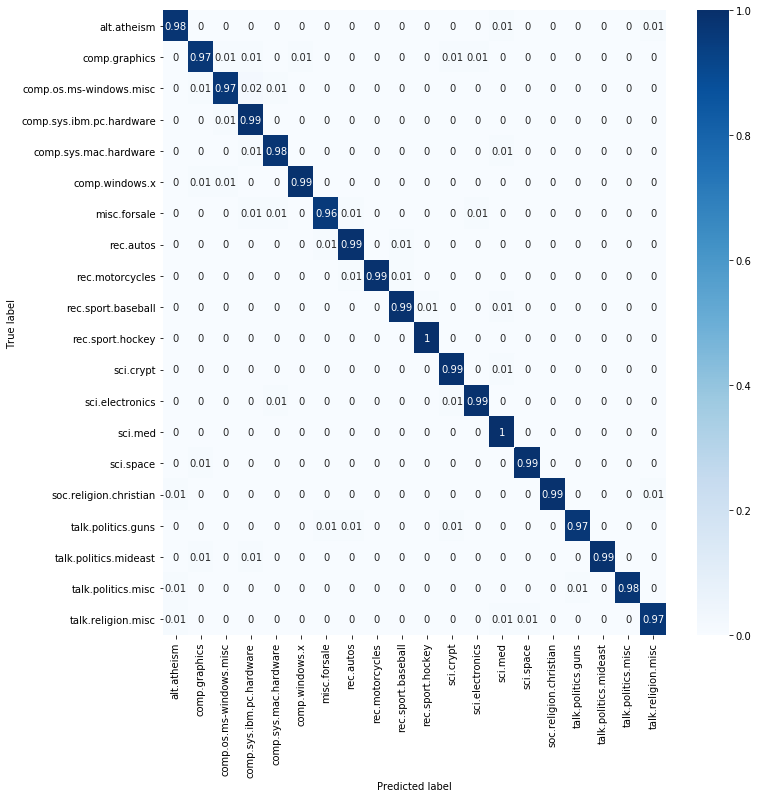
\includegraphics[width=0.6\textwidth]{tfidf_matrix.png}
    \end{frame}


    \section{Reccurent Neural Network approach}
    \begin{frame}
    	\frametitle{Next chapter}
        \tableofcontents[currentsection]
    \end{frame}
    \begin{frame}
        \frametitle{Embedding}
        Popular method in recommendation algorithms (e.g. YouTube)
        Words or phrases from the vocabulary are mapped to vectors of real numbers. E. g. \\
        \begin{center}
            'word' = [2.23, 33., 0.2, ...]
        \end{center}
        Used also as a dimensionality reduction technique.
        \begin{itemize}
            \item $f(w) = [x_1, x_2, ... , x_n]$
            \item Problem: Minimize a distance between similar/interchangeable words in n-dimensional space (and increase
                distance between unconnected words).
        \end{itemize}
    \end{frame}
    \begin{frame}
        \frametitle{Convolutional Neural Network}
        The Conv Net is a composition of two types of layers:
        \begin{itemize}
            \item Convolutional layers
            \item Pooling layers
        \end{itemize}
        Convolutional NN are able to automated feature extraction from input data (in case of text for e.g. sentece order, words
        co-occurence; in image processing edges, parts of face etc.)
    \end{frame}
    \begin{frame}
    	\frametitle{Recurrent Neural Network}
        \begin{itemize}
            \item Recurrent cells instead of simple neurons (e.g. Long Short Term Memory).
            \item Hidden state handled between timesteps processing.
        \end{itemize}
        RNN can ,,remember'' the context of the text, for instance a gender of a subject. \\
        They are good in predicting time series and generating text based on input words
        (text generators, machine translators, etc.).
    \end{frame}
    \begin{frame}
    	\frametitle{Knowledge transfer}
        \begin{itemize}
            \item Use pre-trained embedding layer as an input for classifier.
            \item Pre-trained Conv layers as input for further layers in Deep NN (popular in image processing).
        \end{itemize}
    \end{frame}
    \begin{frame}
    	\frametitle{Results after training}
        \centering
        Accuracy: \textbf{80,3\%}, F1-Score (weighted): \textbf{93,3\%}
        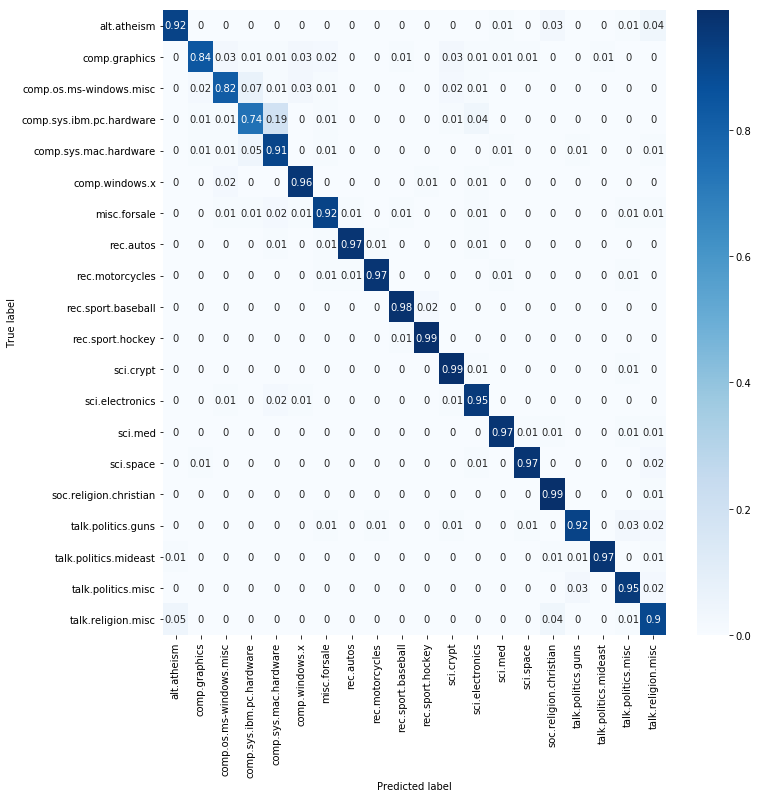
\includegraphics[width=0.6\textwidth]{rnn_matrix.png}
    \end{frame}
    

    \section{Application}
    \begin{frame}
    	\frametitle{Next chapter}
        \tableofcontents[currentsection]
    \end{frame}
    \begin{frame}
    	\frametitle{Application}
        \begin{itemize}
            \item Script written in Python3
            \item Model and parameters exported from Jupiter to external files and loaded during script execution
            \item Simple user interface: \textit{./classifier.py path/to/article.txt}
            \item Result printed in terminal after few seconds
            \item Further steps: 
            \begin{itemize} 
                \item Run script as a service to prevent loading model per each document.
                \item Implement REST API to let other services communicate with the script on demand.
            \end{itemize}
        \end{itemize}
    \end{frame}
    \begin{frame}
    	\frametitle{Thank you!}
        \centering
   	    
\includegraphics[width=0.8\textwidth]{dataScience.png}
    \end{frame}


\end{document}
